%%%%%%%%%%%%%%%%%%%%%%%%%%%%%%%%%%%%%%%%%
% fphw Assignment
% LaTeX Template
% Version 1.0 (27/04/2019)
%
% This template originates from:
% https://www.LaTeXTemplates.com
%
% Authors:
% Class by Felipe Portales-Oliva (f.portales.oliva@gmail.com) with template 
% content and modifications by Vel (vel@LaTeXTemplates.com)
%
% Template (this file) License:
% CC BY-NC-SA 3.0 (http://creativecommons.org/licenses/by-nc-sa/3.0/)
%
%%%%%%%%%%%%%%%%%%%%%%%%%%%%%%%%%%%%%%%%%

%----------------------------------------------------------------------------------------
%	PACKAGES AND OTHER DOCUMENT CONFIGURATIONS
%----------------------------------------------------------------------------------------

\documentclass[
	12pt, % Default font size, values between 10pt-12pt are allowed
	%letterpaper, % Uncomment for US letter paper size
	%spanish, % Uncomment for Spanish
]{../Template/fphw}

% Template-specific packages
\usepackage[utf8]{inputenc} % Required for inputting international characters
\usepackage[T1]{fontenc} % Output font encoding for international characters
\usepackage{mathpazo} % Use the Palatino font

\usepackage{graphicx} % Required for including images

\usepackage{booktabs} % Required for better horizontal rules in tables

\usepackage{listings} % Required for insertion of code

\usepackage{enumerate} % To modify the enumerate environment


% Additional packages needed
\usepackage{amsmath}
\usepackage{enumitem}
\usepackage{mwe}
\usepackage{comment}

\newcommand{\T}{\mathsf{T}}
\newcommand{\E}{\mathbb{E}}

%----------------------------------------------------------------------------------------
%	ASSIGNMENT INFORMATION
%----------------------------------------------------------------------------------------

\title{Homework \#1} % Assignment title

\author{Mao Nishino} % Student name

\date{February 13th, 2024} % Due date

\institute{Florida State University \\ Department of Computer Science} % Institute or school name

\class{Deep and Reinforcement Learning Fundamentals (CAP5619-0001.sp24)} % Course or class name

\professor{Dr. Xiuwen Liu} % Professor or teacher in charge of the assignment

%----------------------------------------------------------------------------------------

\begin{document}

\maketitle % Output the assignment title, created automatically using the information in the custom commands above

%----------------------------------------------------------------------------------------
%	ASSIGNMENT CONTENT
%----------------------------------------------------------------------------------------

\section*{Question 1}

\begin{problem}
	As neural networks are typically trained using (stochastic) gradient descent optimization
algorithms, properties of the activation functions affect the learning. Here we divide the domain of an activation
function into: 1) fast learning region if the magnitude of the gradient is larger than 0.99, 2) active learning region if
the magnitude of the gradient is between 0.01 and 0.99 (inclusive), 3) slow learning region if the magnitude of the
gradient is larger than 0 but smaller than 0.01, and 4) inactive learning region if the magnitude of the gradient is 0.
For each of the following activation functions, \textbf{plot} its gradient in the range from -5 to 5 of the input and then \textbf{list}
the four types of regions. If the gradient is not well defined for an input value, indicate so and then use any reasonable
value.

\begin{enumerate}[label = (\arabic*)]
    \item Rectified linear unit \( f(z) = \begin{cases} z & \text{if } z \geq 0 \\ 0 & \text{otherwise} \end{cases} \)
    \item Logistic sigmoid activation function \( f(z) = \sigma(z) = \frac{1}{1+e^{-z}} \) 
    \item Piece-wise linear unit \( f(z) = \begin{cases} 0.1z+0.9 & \text{if } z> 1 \\ z & \text{if }1\geq z\geq -1 \\ 0.1z-0.9 & \text{Otherwise} \end{cases} \) 
    \item Swish \(f(z) =  z\sigma(2.5z)\), where $\sigma(z) = \frac{1}{1+e^{-z}}$.
    \item Exponential Linear Unit (ELU) \( f(z) = \begin{cases} z & \text{if } z \geq 0 \\ 0.05(e^z-1) & \text{otherwise} \end{cases} \) (Note here is a special case of the general ELU function with $\alpha=0.05$.)
\end{enumerate}

\end{problem}

%------------------------------------------------

\subsection*{Answer}
We will first find the gradients analytically and then show the plot (See Figure \ref{fig:gradients_q1}) and and the list(See Table \ref{tab:q1} ).

\begin{enumerate}[label = (\arabic*)]
\item The gradient of the ReLU function is \( f'(z) = \begin{cases} 1 & \text{if } z > 0 \\ \text{undefined} & z=0\\ 0 & z<0 \end{cases}\). In Figure \ref{fig:gradients_q1}, the value of gradient at $z=0$ is set to be $0$.  
\item By the Chain Rule, the gradient of the logistic sigmoid activation function is $f'(z) = -\frac{1}{(1+e^{-z})^2}\cdot (1+e^{-z})' = -\frac{1}{(1+e^{-z})^2} \cdot (-e^{-z}) = \frac{e^{-z}}{(1+e^{-z})^2} = \sigma(z)(1-\sigma(z))$.
\item The gradient of the piece-wise linear unit is \( f'(z) = \begin{cases} 1 & \text{if } -1<z<1 \\ 0.1 & z>1, z<-1 \\ \text{undefined} & z=-1,1 \end{cases}\). In Figure \ref{fig:gradients_q1}, we will use $1$ for the undefined gradients.
\item In an explicit form, Swish is $f(z) =\frac{z}{1+e^{-2.5z}}$. Therefore, by the Quotient Rule, we have 
\begin{align*}f'(z) &= \frac{1\cdot (1+e^{-2.5z})-z\cdot (-2.5)e^{-2.5z}}{(1+e^{-2.5z})^2} \\ &= \frac{1+e^{-2.5z}+2.5ze^{-2.5z}}{(1+e^{-2.5z})^2}\end{align*}
\item The gradient of the ELU function is \( f'(z) = \begin{cases} 1 & \text{if } z > 0 \\ \text{undefined} & z=0\\ 0.05e^z & z<0 \end{cases}\). In Figure \ref{fig:gradients_q1}, the value of gradient at $z=0$ is set to be $1$. 

\end{enumerate}

Figure \ref{fig:gradients_q1} shows the plot of the gradient for each function along with the list of each activation region. The figure was generated by the notebook \verb|q1figures.ipynb|.

\begin{figure}[!htbp]
    \centering
    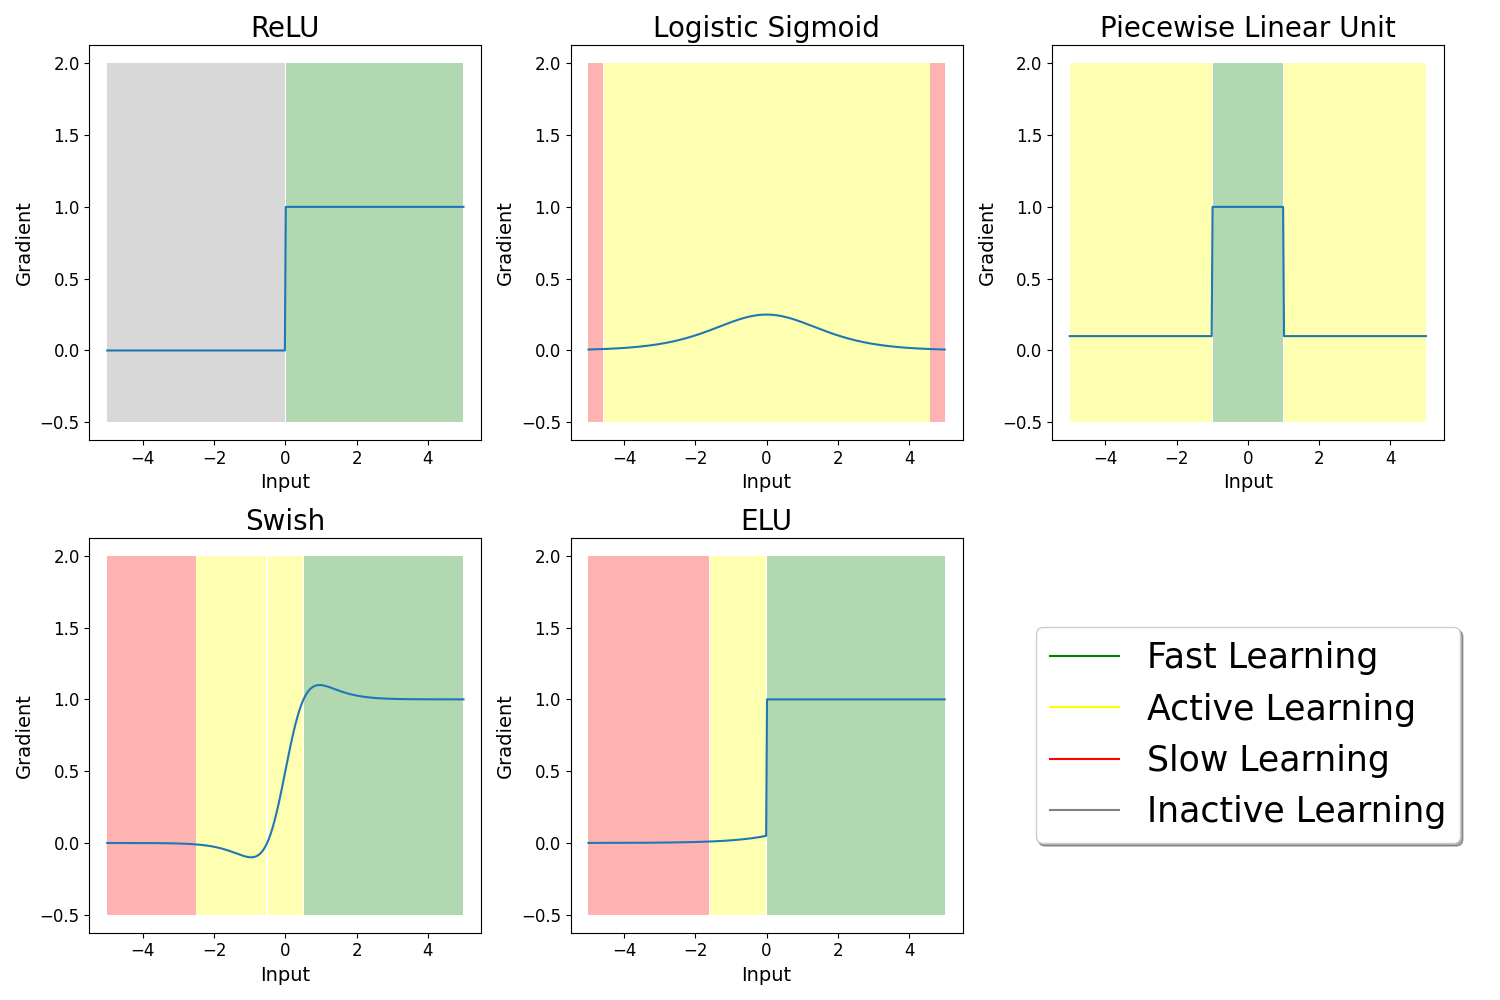
\includegraphics[width=18cm]{HW1/gradient_plot_q1.png}
    \caption{The plot of the gradient of each function.}
    \label{fig:gradients_q1}
\end{figure}

\begin{table}[!htbp]
    \centering
    \begin{tabular}{|c||c|c|c|c|}
        \hline
         Function & Fast  & Active  & Slow & Inactive \\
         \hline
         ReLU & $(0,\infty)$ & $\emptyset$  & $\emptyset$ & $(-\infty,0]$\\
         \hline
         Sigmoid & $\emptyset$ & [-4.58, 4.58]  & (-$\infty$, -4.58)$\cup$ (4.58, $\infty$ ) & $\emptyset$\\
         \hline
         PLU & [-1,1] & (-$\infty$, -1)$\cup$ (1, $\infty$)  & $\emptyset$ & $\emptyset$\\
         \hline
         Swish & (0.49, $\infty$) &  [-2.50,-0.53]$\cup$ [-0.49,0.49] & (-$\infty$,-2.5)$\cup$(-0.53,-0.51)$\cup$(-0.51,-0.49) & $\{-0.51\}$\\
         \hline
         ELU & [0,$\infty$) & [-$\log{5}$,0)  & (-$\infty$, -$\log{5}$) & $\emptyset$\\
         \hline
    \end{tabular}
    \caption{The actiavtion regions for each function. The decimals are rounded to the nearest hundredth.}
    \label{tab:q1}
\end{table}

%----------------------------------------------------------------------------------------

\section*{Question 2}

\begin{problem}
Using a deep learning framework you have established, design and train a fully connected
ReLU neural network to approximate the following function:
\begin{equation}
    g(x) = \sin\left(\frac{\pi}{4}x\right)
\end{equation}
Here all the activation functions in the neural network are ReLU except the output layer, where the linear function
is used. Note that your neural network should have as few as possible neurons in the hidden layer(s) and the
largest error (i.e., the absolute difference between g(x) and the output of your neural network) should be no more
than 0.05 in the range of inputs from -2 to 2. You can generate and use no more than 200 training samples.
(a) Plot the training error with respect to the epoch along with the average and maximal error of the network
at the end of the epoch for the inputs from -2 to 2.
(b) Note that nonlinearity is essential for (deep) neural networks as one with no nonlinearity is reduced to a
one-layer neural network. The nonlinearity of every ReLU neural network can be characterized using
activation patterns, along with the activation regions. For any valid input, the activation pattern of a ReLU
network is a binary string for all its ReLU neurons, where 1 is assigned to such a neuron whose gradient is
1 and 0 is assigned to such a neuron whose gradient is 0. An activation region consists of all the inputs
with the same binary activation string. Compute the activation regions for your trained network and color
them for the inputs from -2 to 2. For each activation region, give its activation pattern.
(c) One way to characterize the dynamics of a neural network during training is to quantify the activation
pattern changes. At the beginning and end of each epoch, compute the activation patterns for all the
training examples and then compute the sum of the Hamming distance between the binary activationpatterns at the beginning and end of the epoch over all the training samples. Then plot the total Hamming
distance with respect to the training epoch. Is the overall trend consistent with your expectation? Provide a
justification.
\end{problem}

%------------------------------------------------

\subsection*{Answer}
For the following results, refer to \verb|q2main.ipynb| for the code. We have used 1-layer (excluding the input layer) neural nets for this problem. To find out the number of neurons needed, we calculated the maximal absolute error between $g(x)$ and our neural nets for the test samples (generated from $1000$ points in the interval $[-2,2]$) at the end of the training for each number of neurons. As a result, we have found that the 1-layer NN with two neurons achieves the maximal absolute error of \verb|0.10111761|, while the NN with three neurons achieved \verb|0.04396987|, which is below the required threshold. Therefore, we will use this three-layer NN for the subsequent problems. The models we mentioned above are included in the \verb|code| folder, with the file name \verb|net_2.pt| for two neurons NN and \verb|net_3.pt| for three neurons NN. For the training, we used the SGD with momentum using the learning rate $0.01$ and the momentum constant $0.1$.

\begin{enumerate}[label = (\alph*)]
	\item Figure \ref{fig: q2a} shows the figure for the training error, the average test error, and the maximal test error. 
    \item Figure \ref{fig: q2b} shows the activation regions for each input along with their activation patterns.
    \item Figure \ref{fig: q3} shows the sum of Hamming distances between the activation pattern at the beginning and the end of each epoch. The Hamming distances were calculated using the \verb|spatial.distance.hamming| from \verb|scipy|. The trend is consistent with my expectation that the Hamming distance should eventually be close to zero as the epoch increases. The justification behind this expectation is that the weights should stabilize as they converge, leading to less change before and after an epoch.
\end{enumerate}

\begin{figure}[!htbp]
    \centering
    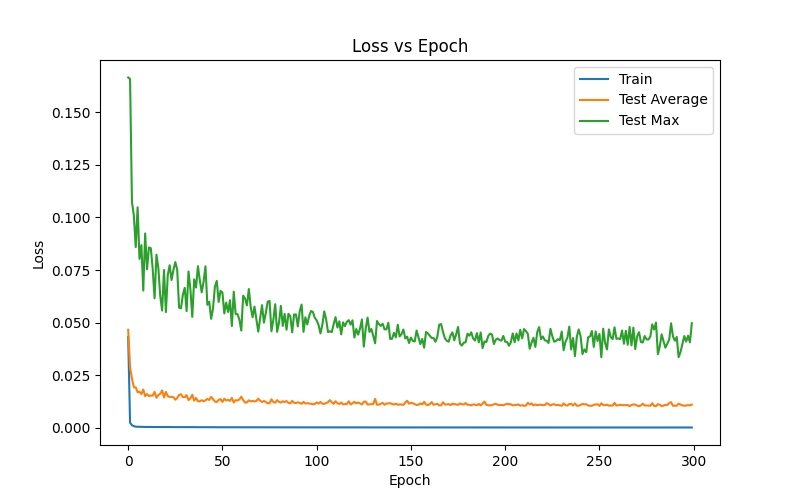
\includegraphics[width=\linewidth]{HW1/q2a.png}
    \caption{The training loss (MSE loss), the maximal absolute test error and the average absolute test error for the three neurons NN.}
    \label{fig: q2a}
\end{figure}

\begin{figure}[!htbp]
    \centering
    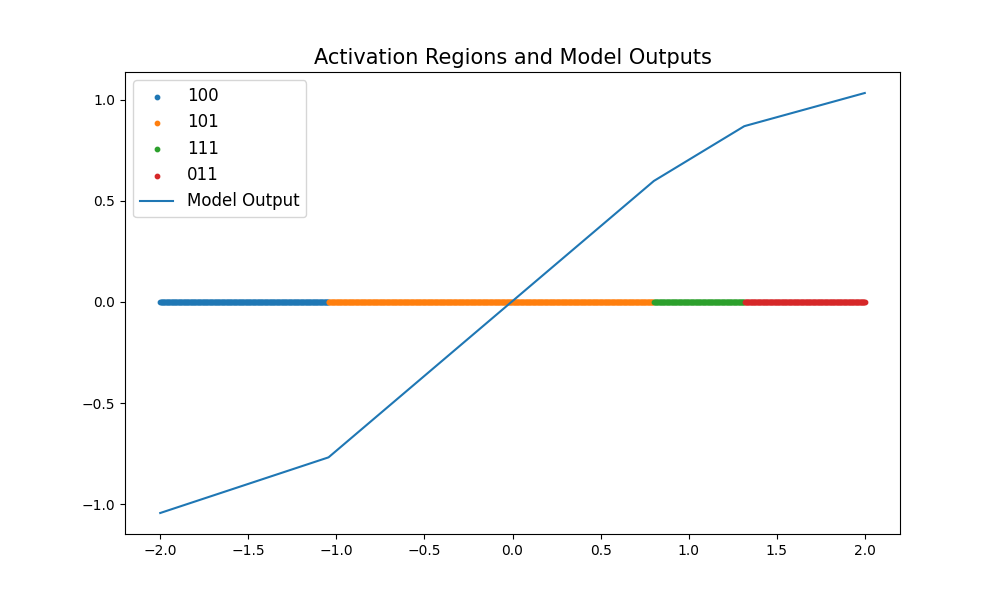
\includegraphics[width=\linewidth]{HW1/q2b.png}
    \caption{The activation regions for each input along with its output from the trained NN. The legend shows the activation patterns for each region.}
    \label{fig: q2b}
\end{figure}

\begin{figure}[!htbp]
    \centering
    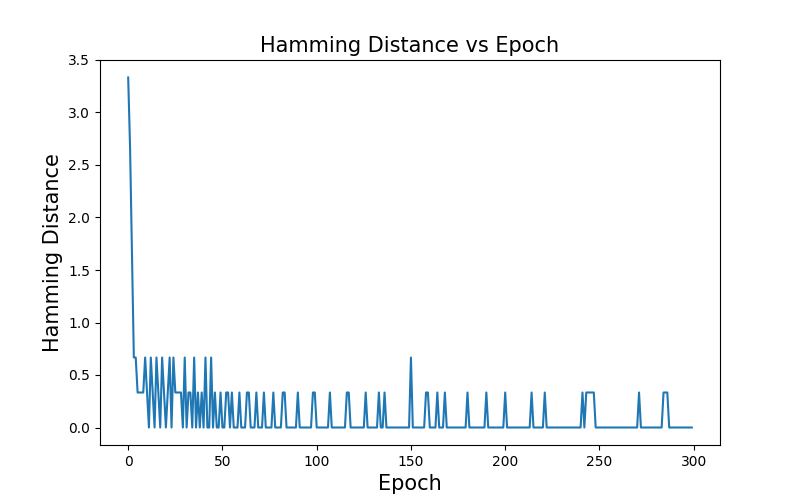
\includegraphics[width=0.9\linewidth]{HW1/q3.png}
    \caption{The sum of Hamming distances at each epoch. We observe that the quantity will be close to zero as the model converges. We observe some oscillations from stochastic noise generated by SGD, but overall, the trend fits our expectations.}
    \label{fig: q3}
\end{figure}
%----------------------------------------------------------------------------------------

\section*{Question 3}

\begin{problem}
The weights and biases of a softmax layer (implemented using equations (6.28) and (6.29)
in
the
Deep
textbook)
can
be
downloaded
from
http://www.cs.fsu.edu/\~liux/courses/deepRL/assignments/hw2\_softmax\_weights.m. (Note that they are given as a
Matlab program and you need to extract the numbers from the file.)
\begin{enumerate}[label=(\arabic*)]
\item (2 points) What is the architecture of the softmax layer? In other words, how many inputs, how many
neurons, and how many connections are there in the layer?
\item (4
points)
Classify
the
following
example,
which
can
be
downloaded
from
http://www.cs.fsu.edu/~liux/courses/deepRL/assignments/hw2\_softmax\_sample.txt .
\item (8 points) Suppose that we use cross entropy loss, the learning rate is 0.1, and the correct label for the
sample is the sixth class (i.e., class 5 if you labels the classes as 0, 1, 2, ..., 19), after we apply one step
gradient decent optimization using the given sample in (2), how many of the weights and biases will be
increased, decreased, or remain the same respectively? For numerical stability, we consider any change
smaller than 0.00001 as "remining the same."
\item (6 points) Compute a small vector so that the new sample created by adding the vector to the given sample
will be classified as from the sixth class (i.e., class 5 if you label the classes as 0, 1, ..., 19). The length of
the vector (in L 2 norm) should be as small as possible. Explain how you have obtained your solution and
confirm that the resulting sample is indeed classified as from the sixth class. (Note: in the literature, such
examples are known as adversarial examples. Hint: any reasonable way to compute the change vector will
be accepted; to compute the optimal solution, you need to formulate it as a quadratic optimization problem,
that is, to minimize the square of the length of the vector under the constraints the output from the sixth
class is the largest.)
\end{enumerate}


\end{problem}

\begin{problem}
    (5) (extra credit option 3 points) As in (4), could you make a small change to the given sample so that it will
be classified as from the sixth class but with the maximal changed value to be minimized? In other words,
we like the vector to be as small as possible according to the $L^{\infty}$ norm. Explain how you have obtained your
solution and confirm that the resulting sample is indeed classified as from the sixth class. (Hint: to compute
the optimal solution, you need to formulate it as a linear programming problem by introducing an auxiliary
variable.)
\end{problem}

%------------------------------------------------

\subsection*{Answer} Refer to \verb|q3main.ipynb| for the codes used in this problem.
\begin{enumerate}[label = (\arabic*)]
    \item The number of biases in the layer is $20$, indicating 20 neurons. The shape of the weights array is (100, 20), indicating 100 inputs. The number of connections is the product of them, which is $20\cdot 100=2000$. 
    \item Suppose we label the classes as 0, 1, 2, ..., 19. Then, the class of the sample given is 3 (i.e., the fourth class). Figure \ref{fig:q42} shows the predicted probability from each class.
    \begin{figure}[!htbp]
        \centering
        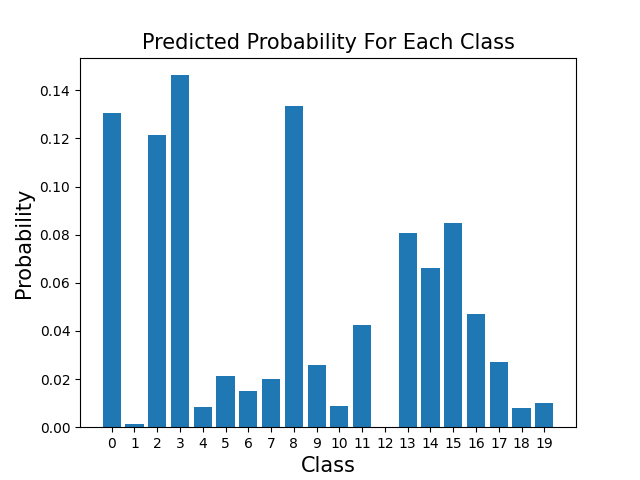
\includegraphics{HW1/q4-2.png}
        \caption{The predicted probability for the given sample using the given softmax layer. The figure clearly indicates that the class 3 has the highest probability.}
        \label{fig:q42}
    \end{figure}
    \item By using a \verb|PyTorch| code, we found that 10 weights increased, 180 decreased, and 1810 remained the same. For biases, 1 bias increased, 18 decreased, and 1 stayed the same.
    \item Supose $p(x,i)$ is the output of the softmax layer for class $i$ where $i=0,\cdots 19$ for a sample $x$. The problem we want to solve is 
    \begin{align}
        &\textrm{minimize } \|\Delta x\|^2_{L^2} \\
        &\textrm{subject to } p(x_0+\Delta x, 5) \geq p(x_0+\Delta x, i), i=0,\cdots ,19 \label{eqn: max_constraint}
    \end{align}
    where $x_0$ is the given sample. Since (\ref{eqn: max_constraint}) is equivalent to the fact that the cross-entropy loss for the class 5 is minimal, as an approximation for this optimization problem, we solve the following:
    \begin{align}
        &\textrm{minimize } \|\Delta x\|^2_{L^2} -\log{p(x+\Delta x, 5})
    \end{align}
    where $-\log{p(x+\Delta x, 5}) $ is the cross-entropy loss for class 5. We will solve this optimization problem using the L-BFGS algorithm. In particular, we use the \verb|fmin_l_bfgs_b| function from \verb|scipy|. This is the adaption of the method mentioned in \cite{szeg}. Figure \ref{fig:q4-4} shows the predicted probability for $x_0+\Delta x$ where $\Delta x$ is the solution to the optimization problem. As the figure shows, the sample is now predicted to be in class 5.
    \begin{figure}[!htbp]
        \centering
        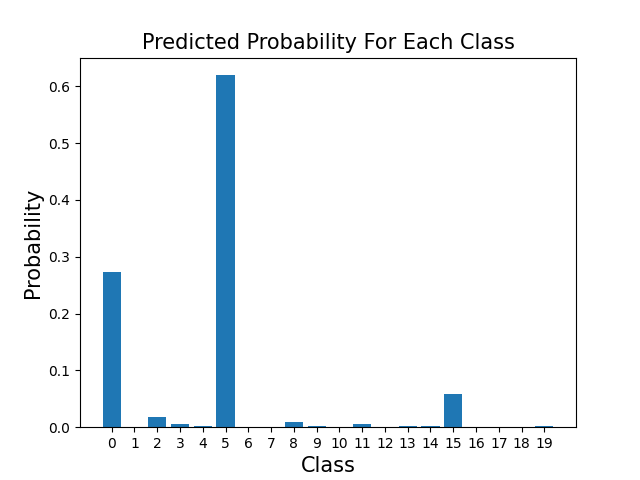
\includegraphics{HW1/q4-4.png}
        \caption{Predicted probabilities for $x_0+\Delta x$. Not only is the predicted class 5, but it is also dominating other classes.}
        \label{fig:q4-4}
    \end{figure}
    \item The problem we would like to solve is the following.     \begin{align}
        &\textrm{minimize } \|\Delta x\|_{L^\infty} \\
        &\textrm{subject to } p(x_0+\Delta x, 5) \geq p(x_0+\Delta x, i), i=0,\cdots ,19
    \end{align}
    This problem is equivalent to the following "epigraph form":
        \begin{align}
        &\textrm{minimize } &t \\
        &\textrm{subject to } &p(x_0+\Delta x, 5) \geq p(x_0+\Delta x, i), i=0,\cdots ,19  \\
        & & \|\Delta x\|_{L\infty}\leq t
    \end{align}
    which is equivalent to
    \begin{align}
        &\textrm{minimize } &t \\
        &\textrm{subject to } &p(x_0+\Delta x, 5) \geq p(x_0+\Delta x, i), i=0,\cdots ,19  \\
        & & \forall i, \Delta x_i -t \leq 0\\
        & & \forall i, -\Delta x_i -t \leq 0
    \end{align}
    Here, both $t$ and $\Delta x$ are optimization variables. We will now analyze the class constraint $p(x_0+\Delta x, 5) \geq p(x_0+\Delta x, i)$. We note that the analytic form for $p(x,i)$ is
    \begin{align}
        p(x,i) = \textrm{SoftMax}(w^T_ix+b_i) = \frac{\exp(w^T_ix+b_i)}{\sum_{i}\exp(w^T_ix+b_i)}
    \end{align}
    where $w_i$ and $b_i$ are the weight and the bias for the neuron $i$. Therefore, for each $i$, $p(x_0+\Delta x,5)\geq p(x_0+\Delta x, i)$ is equivalent to
    \begin{align}
        \frac{\exp(w^T_5(x_0+\Delta x)+b_5)}{\sum_{i}\exp(w^T_i(x_0+\Delta x)+b_i)} \geq \frac{\exp(w^T_i(x_0+\Delta x)+b_i)}{\sum_{i}\exp(w^T_i(x_0+\Delta x)+b_i)} \\
        \exp(w^T_5(x_0+\Delta x)+b_5) \geq\exp(w^T_i(x_0+\Delta x)+b_i) \\
        w^T_5(x_0+\Delta x)+b_5 \geq w^T_i(x_0+\Delta x)+b_i \\
        (w^T_5-w^T_i)(x_0+\Delta x)+(b_5-b_i)\geq 0 \\
        (w_5-w_i)^T \Delta x + (b_5-b_i) + (w_5-w_i)^Tx_0 \geq 0
    \end{align}
    As we can see, the constraint defines a linear (or rigorously, an affine) region on $\Delta_x$ space. The complete linear programming problem we would like to solve is the following:
    \begin{align}
        &\textrm{minimize } &t \\
        &\textrm{subject to } &\forall i, (w_i-w_5)^T \Delta x \leq -(b_i-b_5) - (w_i-w_5)^Tx_0  \\
        & & \forall i, \Delta x_i -t \leq 0\\
        & & \forall i, -\Delta x_i -t \leq 0
    \end{align}
    To solve the problem numerically, we need to write our problem as the standard form of linear programming. For $\Delta x\in \mathbb{R}^{100}$ and $t\in \mathbb{R}$, define:
    \begin{align}
        c &= \begin{pmatrix}\textbf{0}_{100} \\ 1\end{pmatrix}\\
        v &= \begin{pmatrix} \Delta x \\ t \end{pmatrix} \\
        A &= \begin{pmatrix}
            (w_0-w_5)^T & 0 \\
            \vdots & \vdots \\
            (w_{19}-w_5)^T & 0 \\
            \textbf{E}_{100\times 100} & -\textbf{1}_{100} \\
            -\textbf{E}_{100\times 100} & -\textbf{1}_{100}
        \end{pmatrix} \\
        u &= \begin{pmatrix}-(b_0-b_5) - (w_0-w_5)^T x_0 \\ \vdots \\ -(b_{19}-b_5) - (w_{19}-w_5)^T x_0 \\ \textbf{0}_{200}\end{pmatrix}
    \end{align}
    where $\textbf{0}_{n}$ is the $n$ dimensional vector with zeros, $\textbf{1}_n$ is the analogous vector for ones, and $\textbf{E}_{100\times 100}$ is the $100\times 100$ identity matrix. Then our problem becomes
    \begin{align}
        &\textrm{minimize } c^T v \\
        &\textrm{subject to }  Av \leq u
    \end{align}
    which is the standard form of linear programming. We will now solve the problem using the \verb|linprog| function on \verb|scipy|. Figure \ref{fig:q4-5} shows the predicted probability for the adversarial example generated. We note that class 0 and class 5 achieve the same probability up to numerical precision, and thus, the example can be classified as class 0 and class 5. However, by slightly increasing the magnitude of $\Delta x$, we can observe that our example will indeed be classified as class 5 and nothing else. This shows that our $\Delta x$ has the minimal magnitude to satisfy the constraint and that $x_0+\Delta x$ works as the adversarial example.
    \begin{figure}[!htbp]
        \centering
        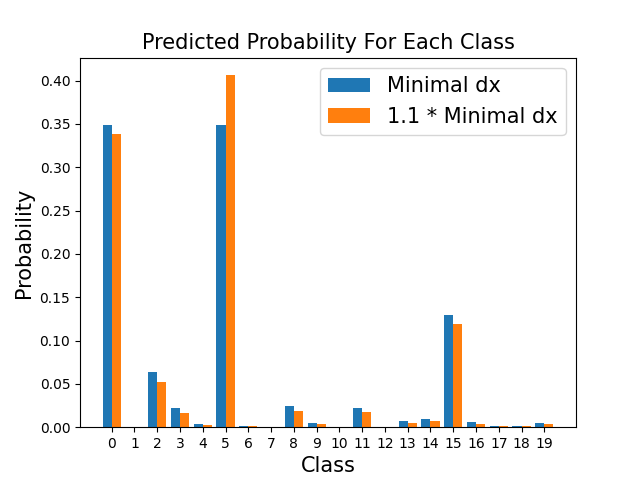
\includegraphics[width=\linewidth]{HW1/q4-5.png}
        \caption{The predicted probability for $x_0+\Delta x$ and $x_0+1.1\Delta x$ where $\Delta x$ is the solution for the linear programming problem. By the standard fact about linear programming, $\Delta x$ lies on the boundary of our constrained space, meaning that our adversarial example is "almost" classified as another class (class 0 in our case). We can also see that the higher probability on class 5 is not a coincidence by slightly increasing the magnitude of $\Delta x$, which can be seen in the figure.}
        \label{fig:q4-5}
    \end{figure}
\end{enumerate}

\section*{Question 4}

\begin{problem}
In the paper “Distributed Representations of Words and Phrases and their Compositionality”
(which can be downloaded from https://papers.nips.cc/paper/5021-distributed-representations-of-words-andphrases-and-their-compositionality.pdf), an objective function based on negative sampling is defined (see Equation
(4) in the paper).
(1) (2 points) Suppose that we use k negative samples to approximate the expectation, write down the objective
function for one sample. Make sure that you define/explain all the variables in your function.
(2) (2 points) Derive the learning rule using gradient descent for the objective function given in (1).
(3) (1 point) Explain the key differences between the learning rule for part (2) and the one we derived in class
for the skip gram model; if you think that the two learning rules are equivalent, justify your answer.

\end{problem}

\subsection*{Answer}
\begin{enumerate}[label=(\arabic*)]
    \item We interpret the problem as follows: We write down an objective function for one specific word $w_t$. Then, the objective function is 
    \begin{equation}
        -\left(\sum_{-c\leq j\leq c, j\neq 0}\log{\sigma(v'^\T_{w_{t+j}} v_{w_t})} + 2c\sum_{j=1}^{k}\log{\sigma(-v'^\T_{n_t^j} v_{w_t})}\right) \label{eqn: objective_ns}
    \end{equation}
    Here, $w_1,\cdots w_T$ is the training data of size $T$, $c$ is the window size, $v_{w}'$ is the output representation of the word $w$, $v_w$ is the input representation of the word $w$, $\sigma(z)$ is the sigmoidal function, $v^\T$ represents the transpose of the vector $v$, and $n_t^j$ is the $j$th negative sample corresponding to the center word $w_t$.

    \item Denote the objective in (\ref{eqn: objective_ns}) as $E$. We consider two cases.
        \begin{enumerate}[label=(\roman*)]
            \item The case for the input representation. The derivative of $E$ with respect to $v_{w_t,i}$ (the $i$th element of the vector $v_{w_t}$) is
            \begin{align}
                \frac{\partial E}{\partial v_{t,i}} &= -\left(\sum_{-c\leq j \leq c, j\neq 0}  \frac{\sigma'(v'^\T_{w_{t+j}} v_{w_t})}{\sigma(v'^\T_{w_{t+j}} v_{w_t})}v'_{w_{t+j},i}+2c\sum_{j=1}^{k}\frac{\sigma'(-v'^\T_{n_t^j} v_{w_t})}{\sigma(-v'^\T_{n_t^j} v_{w_t})}(-v'_{n_t^j,i}) \right) \\ &= -\left(\sum_{-c\leq j \leq c, j\neq 0}  (1-\sigma(v'^\T_{w_{t+j}} v_{w_t}))v'_{w_{t+j},i}-2c\sum_{j=1}^{k}(1-\sigma(-v'^\T_{n_t^j} v_{w_t}))v'_{n_t^j,i} \right) \\ &=-\left(\sum_{-c\leq j \leq c, j\neq 0}  (1-\sigma(v'^\T_{w_{t+j}} v_{w_t}))v'_{w_{t+j},i}-2c\sum_{j=1}^{k}\sigma(v'^\T_{n_t^j} v_{w_t})v'_{n_t^j,i} \right)
            \end{align}
            Therefore, the update rule by the gradient descent is
            \begin{equation}
                v_{w_t,i}^{new} = w_{w_t,i}+\eta\left(\sum_{-c\leq j \leq c, j\neq 0}  (1-\sigma(v'^\T_{w_{t+j}} v_{w_t}))v'_{w_{t+j},i}-2c\sum_{j=1}^{k}\sigma(v'^\T_{n_t^j} v_{w_t})v'_{n_t^j,i} \right)
            \end{equation}
            or equivalently,
            \begin{equation}
                v_{w_t}^{new} = v_{w_t}+\eta\left(\sum_{-c\leq j \leq c, j\neq 0}  (1-\sigma(v'^\T_{w_{t+j}} v_{w_t}))v'_{w_{t+j}}-2c\sum_{j=1}^{k}\sigma(v'^\T_{n_t^j} v_{w_t})v'_{n_t^j} \right)
            \end{equation}
            where $\eta$ is the learning rate.
            \item The case for the output representation. The derivative of $E$ with respect to $v_{w_s,i}'$ (the $i$th element of the vector $v_{w_s}'$) is
            \begin{align}
                \frac{\partial E}{\partial v_{w_s,i}'} &= -\left(\sum_{\substack{-c\leq j \leq c, j\neq 0, \\ w_{t+j}=w_s}}\frac{\sigma'(v'^\T_{w_{t+j}} v_{w_t})}{\sigma(v'^\T_{w_{t+j}}v_{w_t})} v_{w_t,i}+2c \sum_{\substack{j=1 \\n_t^{j}=w_s}}^{k}\cdot\frac{\sigma'(-v'^\T_{n_t} v_{w_t})}{\sigma(-v'^\T_{n_t} v_{w_t})}(-v_{w_t,i}) \right) \\ &=-\left(\sum_{\substack{-c\leq j \leq c, j\neq 0, \\ w_{t+j}=w_s}}(1-\sigma(v'^\T_{w_{t+j}} v_{w_t})) v_{w_t,i}-2c\sum_{\substack{j=1\\n_t^j = w_s}}^k\sigma(v'^\T_{n_t^j} v_{w_t})v_{w_t,i} \right)
            \end{align}
            Therefore, the update rule is
            \begin{equation}
                v_{w_s,i}'^{new} = w_{w_s,i}'+ \eta\left(\sum_{\substack{-c\leq j \leq c, j\neq 0, \\ w_{t+j}=w_s}}(1-\sigma(v'^\T_{w_{t+j}} v_{w_t})) v_{w_t,i}-2c\sum_{\substack{j=1\\n_t^j = w_s}}^k\sigma(v'^\T_{n_t^j} v_{w_t})v_{w_t,i} \right)
            \end{equation}
            or equivalently,
            \begin{equation}
                v_{w_s}'^{new} = w_{w_s}'+ \eta\left(\sum_{\substack{-c\leq j \leq c, j\neq 0, \\ w_{t+j}=w_s}}(1-\sigma(v'^\T_{w_{t+j}} v_{w_t})) v_{w_t}-2c\sum_{\substack{j=1\\n_t^j = w_s}}^k\sigma(v'^\T_{n_t^j} v_{w_t})v_{w_t} \right)
            \end{equation}
            \end{enumerate}
    \item In both the input and output update rule, the training stops when $\sigma(v'^\T_{w_{t+j}} v_{w_t}) \sim 1$ and $\sigma(v'^\T_{n_t} v_{w_t}) \sim 0$. This means that the update rule tries to make context words as close as possible and make noises and context words as far as possible in terms of cosine similarity. This is fundamentally different from the original Skip-Gram model, where we do not try to distinguish the noise.
    
\end{enumerate}



\begin{comment}
%----------------------------------------------------------------------------------------

\section*{Question 4 }

\begin{problem}
	The table below shows the nutritional consistencies of two sausage types. Explain their relative differences given what you know about daily adult nutritional recommendations.
	
	\bigskip
    
	\begin{center}
		\begin{tabular}{l l l}
			\toprule
			\textit{Per 50g} & Pork & Soy \\
			\midrule
			Energy & 760kJ & 538kJ\\
			Protein & 7.0g & 9.3g\\
			Carbohydrate & 0.0g & 4.9g\\
			Fat & 16.8g & 9.1g\\
			Sodium & 0.4g & 0.4g\\
			Fibre & 0.0g & 1.4g\\
			\bottomrule
		\end{tabular}
	\end{center}
	
	\medskip
\end{problem}



%------------------------------------------------

\subsection*{Answer}

Lorem ipsum dolor sit amet, consectetur adipiscing elit. Praesent porttitor arcu luctus, imperdiet urna iaculis, mattis eros. Pellentesque iaculis odio vel nisl ullamcorper, nec faucibus ipsum molestie. Sed dictum nisl non aliquet porttitor. Etiam vulputate arcu dignissim, finibus sem et, viverra nisl. Aenean luctus congue massa, ut laoreet metus ornare in. Nunc fermentum nisi imperdiet lectus tincidunt vestibulum at ac elit. Nulla mattis nisl eu malesuada suscipit.

%----------------------------------------------------------------------------------------

\section*{Question 5 (bonus marks)}

\begin{problem}
	\lstinputlisting[
		caption=Luftballons Perl Script, % Caption above the listing
		label=lst:luftballons, % Label for referencing this listing
		language=Perl, % Use Perl functions/syntax highlighting
		frame=single, % Frame around the code listing
		showstringspaces=false, % Don't put marks in string spaces
		numbers=left, % Line numbers on left
		numberstyle=\tiny, % Line numbers styling
	]{}
	
	\begin{enumerate}
		\item How many luftballons will be output by the Listing \ref{lst:luftballons} above?
		\item Identify the regular expression in Listing \ref{lst:luftballons} and explain how it relates to the anti-war sentiments found in the rest of the script.
	\end{enumerate}

\end{problem}

%------------------------------------------------

\subsection*{Answer}

\begin{enumerate}
	\item 99 luftballons.
	\item Lorem ipsum dolor sit amet, consectetur adipiscing elit. Praesent porttitor arcu luctus, imperdiet urna iaculis, mattis eros. Pellentesque iaculis odio vel nisl ullamcorper, nec faucibus ipsum molestie. Sed dictum nisl non aliquet porttitor. Etiam vulputate arcu dignissim, finibus sem et, viverra nisl. Aenean luctus congue massa, ut laoreet metus ornare in. Nunc fermentum nisi imperdiet lectus tincidunt vestibulum at ac elit. Nulla mattis nisl eu malesuada suscipit.
\end{enumerate}

%----------------------------------------------------------------------------------------
\end{comment}

\begin{thebibliography}{9}
\bibitem{szeg}
Szegedy, C., Zaremba, W., Sutskever, I., Bruna, J., Erhan, D., Goodfellow, I., \& Fergus, R. (2014). Intriguing properties of neural networks. arXiv:1312.6199 [cs.CV].

\end{thebibliography}

\end{document}

    \begin{comment}
        \begin{enumerate}[label=(\roman*)]
            \item The word $w_{s}$ is not in the training data. In this case, we have
            \begin{align}
                \frac{\partial E}{\partial w_{s,i}} &= \frac{1}{T}\sum_{t=1}^{T}P_n(w_s) \frac{\sigma'(-v'^\T_{w_s}v_{w_t})}{\sigma(-v'^\T_{w_s} v_{w_t})}\cdot (-v_{w_t,i}) \\ &= \frac{1}{T}\sum_{t=1}^{T}P_n(w_s) \frac{\sigma(-v'^\T_{w_s} v_{w_t})(1-\sigma(-v'^\T_{w_s} v_{w_t}))}{\sigma(-v'^\T_{w_s} v_{w_t})}\cdot (-v_{w_t,i}) \\ &= -\frac{1}{T}\sum_{t=1}^{T}P_n(w_s)(1-\sigma(-v'^\T_{w_s} v_{w_t}))v_{w_t ,i}
            \end{align}
            \item The word $w_{s}$ is in the training data. In this case, we have
            \begin{align}
                \frac{\partial E}{\partial w_{s,i}} = \frac{1}{T}\sum_{t=1}^{T}
            \end{align}
        \end{enumerate}
    \end{comment}